\documentclass[11pt,fleqn]{article}

\setlength {\topmargin} {-.15in}
\setlength {\textheight} {8.6in}

\usepackage{amsmath}
\usepackage{amssymb}
\usepackage{color}
\usepackage{tikz}
\usetikzlibrary{automata,positioning,arrows}
\usepackage{diagbox}



\newcommand{\be}{\begin{enumerate}}
\newcommand{\ee}{\end{enumerate}}

\begin{document}
\textbf{Ex 2.2.4:} What happens to merge function if unsorted array? Sort 2 halves, then merge together.(MergeSort)\\

\textbf{Solution:}\\
Worst case is if the subarray is sorted. Global max of one greater than global max of another.

\begin{itemize}
	\item For example, array [1,3,5] AND [2,4,6]
	\item Comparisons go 1 by 1(check top and then bottom, increment top index pointer, then do same process, and increment bottom index pointer until hit the end of both arrays).
	\item So nearly $2n$ comparisons.
	\item If elements of 1 subarray strictly smaller than min of next, then probably take n-compares.
	
\end{itemize}

\begin{center}
 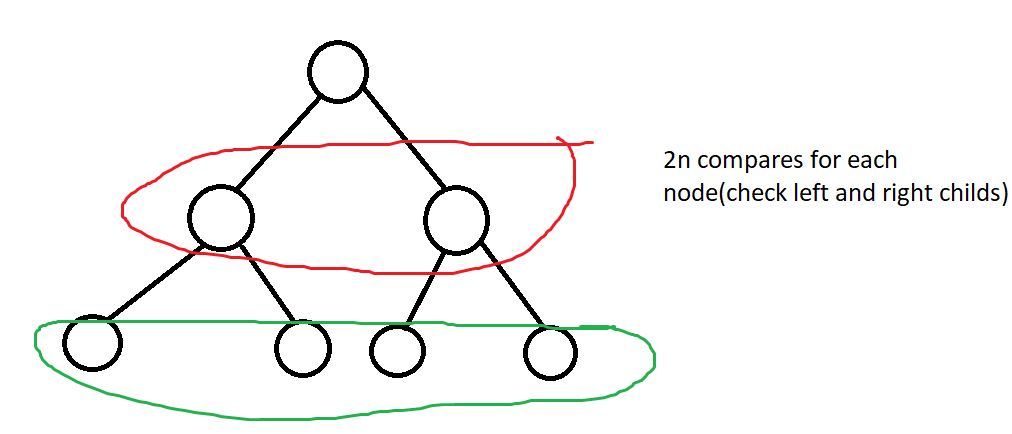
\includegraphics[scale=0.6]{2.2.4.png}
\end{center}
\end{document}
